\chapter{Numerische Quadratur/Integration}

Gegeben: integrierbare Funktion $f: [a,b] \to \R$

\medskip

\emph{Ziel:} Finde $I(f) \colonequals \int_a^b f(x) \; dx$
\begin{satz}[Fundamentalsatz]
Sei $F$ Stammfunktion von $f$, also $F'=f$. Dann ist:
\begin{equation*}
I(f) = F(b) - F(a).
\end{equation*}
\end{satz}
\emph{Aber:} Die Stammfunktion $F$ ist häufig nicht bekannt!

\medskip

\emph{Oder:} $F$ ist schwierig zu handhaben!
\begin{bsp}
\begin{equation*}
f(x) = e^{x^2}
\qquad
F(x) = \sum_{k=0}^\infty \frac{x^{2k +1}}{(2k+1)k!}
\end{equation*}
\end{bsp}
Besser: $I(f)$ numerisch (d.h. approximativ) berechnen.

\bigskip

\emph{Idee:} Wir wissen, wie man Polynome integriert.
\begin{itemize}
\item Sei $\Delta = a \le x_0 < x_1 \dots x_n \le b$ eine Zerlegung des Integrationsgebiets.
\item Sei $p_n$ das dazugehörige Interpolationspolynom von $f$.
\item Approximiere
 \begin{equation*}
  I(f) = \int_a^b f(x) \; dx
  \qquad \text{durch} \qquad
  Q_n(f) \colonequals \int_a^b p_n(x) \; dx.
 \end{equation*}
\end{itemize}
Lagrange-Form von $p_n$:
\begin{equation*}
p_n(x) = \sum_{k=0}^n f(x_k) L_k(x) \; dx
\end{equation*}
Einsetzen ergibt
\begin{align*}
 Q_n(f) = & \int_a^b p_n(x) \; dx = \int_a^b \sum_{k=0}^n f(x_k) L_k(x) \; dx = \sum_{k=0}^{n}f(x_k) \int_a^b L_k(x) \; dx
\\ = & \sum_{k=0}^n f(x_k) a_k,
\end{align*}
mit reellen Koeffizienten $a_k$, die nicht von $f$ abhängen.

\bigskip

Wie genau ist diese Approximation?
\begin{itemize}
\item Wir ahnen schon: es hängt von der Verteilung der Stützstellen ab.
\end{itemize}

\section{Die Newton-Cotes-Formeln}

(Roger Cotes 1682--1716, engl.\ Mathematiker)

\bigskip

Sei $h = \frac{b - a}{n}$ und $x_k = a + hk$.

\medskip

Das dazugehörige $Q_n(\cdot)$ heißt (abgeschlossene) Newton-Cotes-Formel.
\paragraph{Trapezregel:} $n =1$
\begin{itemize}
 \item Stützstellen $x_0 = a, x_1 = b$

 \item Lagrange-Polynome:
\begin{align*}
L_0(x) = \frac{x-x_1}{x_0 - x_1} = \frac{b-x}{h}
\qquad
L_1(x) = \frac{x-x_0}{x_1 - x_0} = \frac{x-a}{h}
\end{align*}
\item Integrale der Lagrange-Polynome
\begin{align*}
\int_a^bL_0(x) \; dx = & \frac{1}{h} \int_a^b b-x \; dx = \frac{1}{h} \Big(bx - \frac{x^2}{2}\Big)\bigg\vert^b_a
\\ = & \frac{1}{h} \Big[ b^2 - \frac{b^2}{2} - ab + \frac{a^2}{2} \Big] = \frac{1}{2h} (b-a)^2 = \frac{h}{2}
\end{align*}
 und
 \begin{equation*}
\int_a^b L_1(x) \; dx = \frac{h}{2}.
\end{equation*}
 \item Also: \begin{equation*}
Q_1(f) = f(x_0) \int_a^b L_0(x) \,dx + f(x_1)\int_a^b L_1(x) \,dx = \frac{h}{2} f(x_0) + \frac{h}{2} f(x_1).
\end{equation*}
\end{itemize}

\paragraph{Simpson-Regel:} $n=2$
\begin{equation*}
Q_2(f) = \frac{h}{6} f(x_0) + \frac{4h}{6} f(x_1) + \frac{h}{6} f(x_2)
\end{equation*}

\section{Quadraturfehler der Simpson-Regel}
\begin{satz}
Sei $f \in C^4[a,b]$. Dann ist
\begin{equation*}
\abs{Q_2(f) - I(f)} \le \frac{1}{12} h^5 \norm{ f^{(4)} }_\infty.
\end{equation*}
\end{satz}
[Wenig überraschend: Polynome vom Grad $\le 3$ werden exakt integriert.]

\todoannot{\baselineskip}{Prüfen: Bei Dd steht sogar 1/90.}

\begin{proof}
\begin{itemize}
\item Wir benutzen die Hilfsfunktion aus Satz~\ref{thm:interpolation:interpolation_error}
\begin{equation*}
w(x) \colonequals (x-a)(x-x_1)(x-b) = (y+h)\;y\; (y-h)
\end{equation*}
mit $y \colonequals x - x_1$.

 \item Das Integral davon ist
  \begin{equation*}
   W(h) \colonequals \int_{-h}^h (y+h) \;y\; (y-h) \,dy = 0
  \end{equation*}
  da der Integrand ungerade ist.
\end{itemize}

\bigskip

Jetzt der Satz~\ref{thm:interpolation:interpolation_error} zum Interpolationsfehler von $p_2$:
\begin{itemize}
 \item Es existiert ein $\xi \in (a,b)$ so dass:
\begin{align*}
f(x) - p_2(x) = &\frac{f'''(\xi)}{3!} w(x)
\end{align*}
\item Integriere über $[a,b]$, und addiere eine Null:
\begin{align*}
\Big\vert \int_a^b \big(f(x) - p_2(x)\big] \, dx \Big\vert
 &=
 \frac{1}{6} f'''(x_1) w(x) + \frac{1}{6} f'''(\xi) w(x) - \frac{1}{6} f'''(x_1)w(x) \\
 &=
 \frac{1}{6}\; \bigg\vert f'''(x_1) \underbrace{\int w(x) \; dx}_{= 0} + \int_a^b \Big(f'''(\xi) - f'''(x_1)\Big) w(x) \, dx \bigg\vert \\
 & \le
 \frac{1}{6} \; \max_{x \in [a,b]} \Big \vert f'''(x) - f'''(x_1) \Big\vert \int_a^b\vert w(x) \vert \, dx.
\end{align*}
\item Mittelwertsatz ($f$ ist $C^4$):

 $\exists \zeta \in (a,b)$ so dass
\begin{equation*}
 \Big\vert f'''(x) - f'''(x_1) \Big \vert
 =
 \big \vert f^{(4)} (\zeta) \big \vert \;\underbrace{\vert x-x_1\vert}_{\le h} \; \le h \norm{f^{(4)}}_\infty.
\end{equation*}
\item Integrals des Betrags der Hilfsfunktion:
\begin{equation*}
 \int_a^b \abs{w(x)}\,dx
 =
 \int_{-h}^h \Big\vert(y+h)\;y \;(y-h)\Big\vert \; dy = -2 \int_0^h (y^2- h^2)y \; dy = \frac{1}{2} h^4
\end{equation*}

\item Deshalb
\begin{align*}
\big \vert Q_2(f) - I(f) \big\vert
 &=
 \Big \vert \int_a^b \big [f(x) - p_2(x) \big] \, dx \Big \vert
\\ \le & \frac{1}{6} h \norm{f^{(4)}}_\infty \underbrace{\int_a^b \vert w(x) \vert \; dx}_{= \frac{1}{2} h^4}
\\ = & \frac{1}{12} h^5 \norm{f^{(4)}}_\infty. \qedhere
\end{align*}
\end{itemize}
\end{proof}

\bigskip

Ähnlich zeigt man:
\begin{lemma}
 Für die Trapezregel $Q_1$ gilt
 \begin{equation*}
  \abs{Q_1(f) - I(f)} \le \frac{1}{12} h^3 \norm{f''}_\infty.
 \end{equation*}
\end{lemma}

Wir haben also

\begin{center}
\begin{tabular}{ c l }
  $Q_1 \rightarrow h^3$ & Trapez-Regel\\
  $Q_2 \rightarrow h^5$ & Simpson \\
  $Q_3 \rightarrow h^?$  & $p=3$ \\
\end{tabular}
\end{center}

Vermutlich liefert $Q_3$ die Konvergenzordnung $h^7$?

\begin{satz}
Sei $Q_n$ die $n$-te Newton-Cotes-Formel
\begin{enumerate}[a)]
\item Falls $n$ gerade und $f \in C^{n+2}$, so existiert ein $\xi \in (a,b)$ so dass
\begin{equation*}
I(f) - Q_n(f) = \frac{h^{n+3}f^{(n+2)}(\xi)}{(n+2)!} \int_0^n t^2(t-1) (t-2) \cdots (t-n) \; dt
\end{equation*}
\item Falls $n$ ungerade und $f \in C^{n+1}$, so existiert ein $\xi \in (a,b)$ so dass
\begin{equation*}
I(f) - Q_n(f) = \frac{h^{n+2}f^{(n+1)}(\xi)}{(n+1)!} \int_0^n t(t-1) (t-2) \cdots (t-n) \; dt
\end{equation*}
\end{enumerate}
\end{satz}
\emph{Moral:} Nur beim Übergang von ungerader zu gerader Ordnung gewinnt man tatsächlich etwas.

\bigskip

Im Prinzip könnte man Formeln immer höherer Ordnung nehmen, und würde immer genauere Approximationen bekommen.

\medskip

\emph{Aber:} Ab $n \ge 7$ bekommt man teilweise negative Gewichte, d.h.
\begin{equation*}
Q_n(f) = \sum_{k=0}^n f(x_k) a_k
\qquad \text{mit} \qquad
a_k = \int_a^b L_k(x) \; dx < 0.
\end{equation*}
Solche Quadraturformeln verletzen die folgende Monotonie des Integrals:
\begin{equation*}
\textnormal{aus } f(x) \ge 0 \quad \forall x \in (a,b)
\qquad \text{folgt} \qquad
\int_a^b f \; dx \ge 0 .
\end{equation*}
Deshalb verwendet man i.A. nur Newton-Cotes-Formeln bis $n=6$.

\section{Zusammengesetzte (summierte) Newton-Cotes-Formeln}
\begin{itemize}
\item Zerlege Intervall in Teilintervalle
\item Quadraturformel niedriger Ordnung auf jedem Teilintervall
\item Zerlege $[a,b]$ in $r$ gleichgroße Stücke der Breite $h \colonequals \frac{b-a}{r}$.
\item Zerlege jedes dieser Stücke wiederum in $n$ gleichgroße Stücke.
\item Zusammengesetzte Trapezregel:
\begin{equation*}
T_h(f) \colonequals \frac{h}{2} \Big(f(x_0) + 2f(x_1) + 2f(x_2) +  \dots + 2f(x_{l-1}) + f(x_{rn}) \big)
\end{equation*}
\item Zusammengesetzte Simpsonregel:
\begin{equation*}
S_h(f) \colonequals \frac{h}{6} \Big(f(x_0) + 4f(x_1) + 2f(x_2) + 4f(x_3) + 2 \dots + 2f(x_{l-2})  + 4f(x_{l-1}) + f(x_{rn}) \big)
\end{equation*}
\end{itemize}

\begin{satz}\mbox{}
\begin{itemize}
\item Für alle $f \in C^2$ gilt
\begin{equation*}
\big\vert T_h(f) - I(f) \big \vert \le \frac{b-a}{12} h^2 \norm{f''}_\infty.
\end{equation*}
\item Für alle $f \in C^4$ gilt
\begin{equation*}
\big\vert S_h(f) - I(f) \big \vert \le \frac{b-a}{180} h^4 \norm{f^{(4)}}_\infty
\end{equation*}
\end{itemize}
\end{satz}

\paragraph{Aufwand:}

Trapezregel \begin{center}
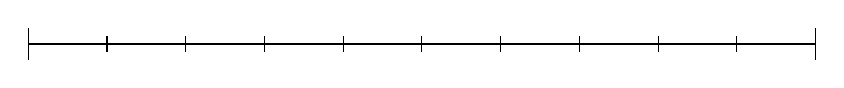
\begin{tikzpicture}[scale =1]
\draw (0,0) -- (10,0);
\draw (0,0.2) -- (0,-0.2);
\draw (10,0.2) -- (10,-0.2);
\foreach \x in {1,2,3,4,5,6,7,8,9}
  \draw (\x,0.1) -- (\x,-0.1);
\end{tikzpicture}
\end{center}
\begin{equation*}
n=1, \qquad  h = \frac{b-a}{r}
\end{equation*}
Simpson
\begin{center}
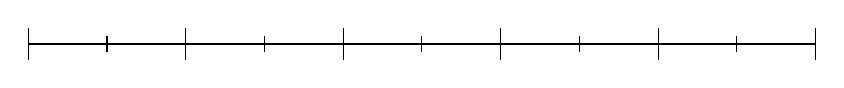
\begin{tikzpicture}[scale =1]
\draw (0,0) -- (10,0);
\foreach \x in {0,2,4,6,8,10}
  \draw (\x,0.2) -- (\x,-0.2);
\foreach \x in {1,3,5,7,9}
  \draw (\x,0.1) -- (\x,-0.1);
\end{tikzpicture}
\end{center}
\begin{equation*}
n=2, \qquad h = 2 h_\text{Trapez}
\end{equation*}
Eine Funktionsauswertung pro Stützstelle:
\begin{itemize}
\renewcommand\labelitemi{$\rightarrow$}
\item Summierte Trapez- \& Simpson-Regel sind in etwa gleich teuer.
\item Aber die summierte Simpson-Regel ist deutlich genauer.
\end{itemize}

\section{Gauß-Quadratur}
Newton-Cotes: Approximiere
\begin{equation*}
 \int_a^b f(x)\,dx
 \qquad \text{durch} \qquad
 \int_a^b p_n(x)\,dx,
\end{equation*}
wobei $p_n$ das Interpolationspolynom $n$-ten Grades \underline{für gleichverteilte Stützstellen} ist.

\bigskip

\emph{Bewiesen:} Diese Approximation ist exakt für alle Polynome vom Grad höchstens $n$.

\medskip

\emph{Bekannt:}
\begin{itemize}
\item Gleichverteilte Stützstellen sind nicht optimal.
\item Können wir mit anderen Stützstellen genauer integrieren?
\item Idealerweise:
\begin{enumerate}[a)]
\item Wir haben $2n +2$ Freiheitsgrade ($n+1$ Werte $+ \;\; n+1$ Pos.)
\item Ein Polynom vom Grad $2n +1$ hat $2n+2$ Koeffizienten
\item[$\Rightarrow$] Wir wollen Polynome vom Grad $2n+1$ exakt integrieren können.
\end{enumerate}
\end{itemize}

\emph{Aber:} Die Positionen der Stützstellen gehen nichtlinear in den Fehler der Quadraturformel ein.

\medskip

Deshalb reicht ein simples Abzählen der Freiheitsgrade nicht aus.

\subsection{Gewichtete Integrale}

Die Gauß-Quadratur wird meistens in einem etwas allgemeineren Kontext eingeführt.
\begin{itemize}
 \item Der Preis für diese zusätzliche Allgemeinheit ist gering.
\end{itemize}

Folgendes Problem wird gelöst:  Wie integrieren wir z.B.\ $\sqrt{x}$?
\begin{itemize}
 \item Diese Funktion hat unbeschränkte Ableitungen!
 \item Die Fehlerabschätzungen sagen deshalb große Quadraturfehler voraus!
\end{itemize}

\emph{Idee:} Gewichtete Integrale

Sei $w: [a,b] \to \R$ eine Gewichtsfunktion, d.h. $w(x) \ge 0$ auf $[a,b]$ und $w(x) > 0$ auf $(a,b)$.

\medskip

Approximiere
\begin{equation*}
 I(f,w) \colonequals \int_a^b f(x)w(x)\,dx
 \qquad \text{durch} \qquad
 \sum_{k=0}^n a_k f(x_k).
\end{equation*}
\emph{Hoffnung:} Nur die Glattheit von $f$ soll in den Fehlerabschätzungen auftauchen.

Die Gewichtsfunktion $w$ muss irgendwie in die Quadraturgewichte $a_k$ einfließen.

\bigskip

\glqq Klassische\grqq{} Gewichte:
\begin{center}
\begin{tabular}{ c | c | l }
   $w$ & $[a,b]$ & Name \\
   \hline
  $1$ & $[-1,1]$ & Gauss--Legendre\\
  $\frac{a}{\sqrt{1-x^2}}$ & $[-1,1]$ &Gauss--Tschebyscheff \\
  $e^{-x^2}$ & $ (-\infty, \infty)$& Gauss--Hermite \\
  $(1-x)^\alpha (1+x)^\beta$, \quad $\alpha, \beta > -1$ & $ [-1,1]$ & Gauss--Jacobi
\end{tabular}
\end{center}

Können wir jetzt die Stützstellen so wählen dass
\begin{equation*}
Q_{n,w}(f) = \int_a^b w(x) f(x) \; dx
\end{equation*}
gilt für \underline{alle} Polynome vom Grad höchstens $2n+1$?

\subsection{Orthogonale Polynome}

Die Geheimwaffe: orthogonale Polynome
\begin{itemize}
\item Das sind Familien von Polynomen
\begin{equation*}
p_0, p_1, p_2, \dots \hspace{2em} p_i \in \Pi_i
\end{equation*}
die paarweise orthogonal sind (bzgl. eines noch zu wählenden Skalarprodukts).
\end{itemize}

\begin{lemma}
Für alle $n \in \N$ sei $Q_{n,w} (\cdot)$ eine Quadraturformel mit Stützstellen
\begin{equation*}
x_{0n} < x_{1n} < \dots < x_{nn}.
\end{equation*}
Für jedes $n \in \N$ definiere das Polynom
\begin{equation*}
p_{n+1}(x) \colonequals (x-x_{0n}) (x-x_{1n}) \dots (x-x_{nn}) \; \in \Pi_{n+1}.
\end{equation*}
Falls $Q_{n,w}$ für alle Polynome aus $\Pi_{2n+1}$ exakt ist, dann steht $p_{n+1}$
$w$-senkrecht auf allen Polynomen niedrigerer Ordnung.  Daraus wiederum folgt
dass  die $p_0, \dots, p_n$ paarweise $w$-orthogonal sind, d.h.
\begin{equation*}
(p_i,p_j)_w \colonequals \int_a^b w(x) p_i(x) p_j(x) \,dx = 0
\qquad
i \neq j, \quad  i,j = 0, \dots, n
\end{equation*}
\end{lemma}
\begin{proof}
Es reicht zu zeigen, dass $(p_j, p_{n+1})_w = 0$ für alle $j < n+1$.
\begin{itemize}
\item Sei also $j<n+1$, und somit $p_j p_{n+1} \in \Pi_{2n+1}$.
\item Rechnen:
\begin{align*}
(p_j, p_{n+1})_w
 & = \int_a^b w p_j p_{n+1}\,dx \\
 & = Q_{n,w} (p_j p_{n+1}) \qquad \qquad \textnormal{da $Q_{n,w}$ exakt auf $\Pi_{2n+1}$} \\
 & = \sum_{k=0}^n a_{kn}p_j(x_{kn})\underbrace{p_{n+1}(x_{kn})}_{= 0} \, dx \\
 & = 0.  \qedhere
\end{align*}
\end{itemize}
\end{proof}
Die gesuchten Knoten $x_{kn}$ müssen also die Nullstellen von Orthogonalpolynomen sein.
\\Gibt es so etwas immer?
\begin{satz}[\citeauthor{deuflhard_hohmann:1993}, Satz~6.2]
Sei $w: (a,b) \to \R$ eine Gewichtsfunktion, so dass
\begin{equation*}
 \norm{p}_w
 \colonequals
 \sqrt{(p,p)_w}
 =
 \sqrt{ \int_a^b w p^2 \, dx} < \infty
\end{equation*}
für alle Polynome $p$. Dann gibt es eine eindeutig bestimmte Familie von Orthogonalpolynomen $p_k \in \Pi_k$ mit führendem Koeffizienten $1$.

Die Polynome genügen der Dreitermrekursion
\begin{equation*}
p_k(x) = (x + \alpha_k) p_{k-1} + \beta_k p_{k-2}(x) \qquad k = 1,2,\dots
\end{equation*}
mit
\begin{equation*}
p_{-1} \colonequals 0, \qquad p_0 \colonequals 1
\end{equation*}
und Koeffizienten
\begin{equation*}
\alpha_k = - \frac{(x p_{k-1}, p_{k-1})_w}{(p_{k-1}, p_{k-1})_w},
\qquad
\beta_k = - \frac{(p_{k-1}, p_{k-1})_w}{(p_{k-2}, p_{k-2})_w}.
\end{equation*}
\end{satz}

\bigskip

Okay, es gibt solche Polynome. Aber kann man die Nullstellen auch wirklich als Quadraturpunkte nutzen?

\begin{satz}[\citeauthor{deuflhard_hohmann:1993}, Satz~6.5]
Das Orthogonalpolynom $p_k \in \Pi_k$ hat genau $k$ einfache Nullstellen in $(a,b)$.
\end{satz}
\begin{proof}\mbox{}
\begin{itemize}
\item Seien $x_1, \dots, x_m$ die $m$ verschiedenen Punkte $x_i \in (a,b)$, an denen $p_k$ sein Vorzeichen wechselt.
\item Zu zeigen: $m \ge k$.
\item Definiere $q(x) \colonequals (x-x_1) \cdots (x-x_m)$
\item $q(x)$ wechselt an den gleichen Stellen sein Vorzeichen.
\item $wqp_k$ wechselt sein Vorzeichen gar nicht!
\item Daraus folgt
 \begin{equation*}
  (q,p_k)_w = \int_a^b wqp_k \,dx \neq 0.
 \end{equation*}
\item $p_k$ steht aber senkrecht auf $\Pi_{k-1}$ (Denn $p_0, \dots, p_{k-1}$ ist Basis von $\Pi_{k-1}$)
\item $q \not\in \Pi_{k-1}$
\item $\Rightarrow m \ge k$ \qedhere
\end{itemize}
\end{proof}


\subsection{Quadratur mit Orthogonalpolynomen}

Wir wissen jetzt
\begin{itemize}
\item $Q_{n,w}$ exakt für $\Pi_{2n +1} \Rightarrow$ Stützstellen sind Nullstellen eines Orthogonalpolynoms.
\end{itemize}

\medskip

Aber gilt auch die andere Richtung?
\begin{itemize}
\item Die Gewichte wählen wir auf jeden Fall wie gehabt:
\begin{equation*}
a_{kn} = \int_a^b L_{kn}(x) \, dx.
\end{equation*}
\end{itemize}
Damit ist die Formel automatisch exakt bis Ordnung $n$.

\bigskip

Das reicht schon!
\begin{lemma}[\citeauthor{deuflhard_hohmann:1993}, Lemma~9.10]
Seien $x_0, \dots, x_n$ die Nullstellen des $(n+1)$-ten Orthogonalpolynoms $p_{n+1}$.
Sei $Q_{n,w}(f) \colonequals \sum_{i=0}^n a_i f(x_i)$ eine beliebige Quadraturformel.
Dann gilt
\begin{equation*}
 \text{$Q_{n,w}$ exakt auf $\Pi_n$}
 \qquad \implies \qquad
 \text{$Q_{n,w}$ exakt auf $\Pi_{2n +1}$}.
\end{equation*}
\end{lemma}
\begin{proof}\mbox{}
\begin{itemize}
\item Sei $Q_{n,w}$ exakt auf $\Pi_n$ und $p \in \Pi_{2n +1}$.
\item Polynomdivision: $\exists q, r \in \Pi_n$ so dass
\begin{equation*}
p = qp_{n+1}  + r.
\end{equation*}
\item $p_{n+1}$ ist $w$-senkrecht zu  $\Pi_n$
\begin{align*}
\Rightarrow \int_a^b wp \,dx
 & =
 \underbrace{\int_a^b wqp_{n+1} \,dx}_{= 0} + \int_a^b wr \,dx = Q_{n,w}(r) \\
 & =
 \sum_{k = 0}^n a_k r(x_k) \\
 & =
 \sum_{k = 0}^n a_k \Big( q(x_k) \underbrace{p_{n+1}(x_k)}_{= 0} + r(x_k)\Big) \\
 & =
 Q_{n,w}(p). \qedhere
\end{align*}
\end{itemize}
\end{proof}

Wie genau ist die Gauss-Quadratur, falls der Integrand kein Polynom in $\Pi_{2n+1}$ ist?

\begin{satz}[\citeauthor{deuflhard_hohmann:1993}, Satz~9.12]
Sei $f \in C^{2n + 2}$. Dann existiert ein $\xi \in [a,b]$ so dass
\begin{equation*}
\int_a^b wf \,dx - Q_{n,w}(f)
=
\frac{f^{(2n+2)}(\xi)}{(2n+2)!} \, \norm{p_{n+1}}^2_w.
\end{equation*}
\end{satz}
Die rechte Seite hängt also tatsächlich nicht von den Ableitungen der Gewichtsfunktion ab!

\bigskip

Die Gauß-Quadratur hat noch einen weiteren wichtigen Vorteil:

\begin{satz}
Alle Gewichte einer Gauss-Formel sind positiv!
\end{satz}
\begin{proof}\mbox{}
\begin{itemize}
\item Sei $q \in \Pi_{2n+1}$ ein Polynom, das nur an einem Knoten $x_k$ nicht verschwindet, also
 \begin{equation*}
  q(x_k) \neq 0
  \qquad \text{und} \qquad
  q(x_i) = 0 \qquad \forall i \neq k.
 \end{equation*}

 \item Wir integrieren dieses Polynom:
  \begin{equation*}
   \int_a^b w q \,dx
   =
   a_k q(x_k)
   \qquad \Rightarrow \qquad
   a_k = \frac{1}{q(x_k)} \int_a^b wq \, dx.
  \end{equation*}

 \item $a_k$ wird positiv wenn $q$ zum Beispiel ein Quadrat ist.

  Wähle ein bestimmtes $q$:
  \begin{align*}
   q(x)
   & \colonequals
   \Big(\frac{p_{n+1}(x)}{x-x_k}\Big)^2 \\
   & =
   (x - x_0)^2 \cdots (x - x_{k-1})^2 (x - x_{k+1})^2 \cdots (x - x_n)^2.
  \end{align*}

 \item Dieses Polynom ist punktweise nicht-negativ, und da die Nullstellen paarweise
   verschieden sind gilt $q(x_k) > 0$.  Deshalb folgt
 \begin{equation*}
  a_k = \frac{1}{q(x_k)} \int_a^b wq \, dx
  > 0. \qedhere
 \end{equation*}
\end{itemize}
\end{proof}

\section{Extrapolationsverfahren für Quadratur}

Idee: Sei $Q_h(f)$ eine Approximation von $I(f)$, die von einem Parameter $h$ abhängt.
\begin{itemize}
\item Annahme: $\lim_{h \to 0} Q_h(f) = I(f)$
\item Berechne zwei (oder mehr) Werte $Q_{h_1}(f)$, $Q_{h_2}(f)$
\item Versuche daraus auf $Q_0(f)$ zu schließen
\begin{center}
    \begin{tikzpicture}
    \draw[->] (-1,0) -- (6.5,0);
    \draw[->] (0,-0.5) -- (0,3);
    \draw (0,0.15) node[left] {$\longrightarrow$};
    \draw (-2.7,0.15) node {extrapoliertes $Q_0(f)$};
    \draw (2,0) node[below] {$h_2$};
    \draw (4.5,0) node[below] {$h_1$};
    \foreach \i in {2,4.5}
        {
            \draw (\i, 0.05) -- (\i,-0.05);
        }
     \draw plot[smooth] coordinates { (0,0.6) (2,0.8) (3.25, 1.1) (4.5,1.6125) (5,1.85) (6,2.4)}; %0.8125/2.5
     \draw (0,0.15) -- (6,2.1); %Steigung ist 0.325
     \draw (2,0.8) node[circle,fill,inner sep=1.5pt]{};
     \draw (4.5,1.6125) node[circle,fill,inner sep=1.5pt]{};
    \end{tikzpicture}
\end{center}
\end{itemize}

Gibt es Quadraturregeln für die diese Extrapolation besonders gut funktioniert?

\subsection{Romberg-Quadratur}

[Nach: Werner Romberg, $1909$ Berlin - $2003$ Heidelberg, emigrierte in die Sowjetunion und Norwegen, Professor in Trondheim und Heidelberg]

\bigskip

Romberg-Quadratur wendet Extrapolation auf die summierte Trapezregel an:
\begin{equation*}
T(h) \colonequals \frac{h}{2} f(a) + h \sum_{i=1}^{n -1} f(a+ ih) + \frac{h}{2} f(b).
\end{equation*}

Um das Fehlerverhalten von $T(h)$ zu verstehen brauchen wir eine asymptotische Entwicklung:
\begin{satz}[\citeauthor{deuflhard_hohmann:1993}, Satz~9.6]
Sei $f \in C^{2m+1}[a,b]$ und $h = \frac{b-a}{n}$ für ein $n \in \N$. Dann gilt für die summierte Trapezsumme
\begin{equation*}
\int_a^b f(x)\;dx = T(h) + c_2h^2 + c_4h^4  + \dots + c_{2m}h^{2m}  + R_{2m+2}(h) h^{2m+2}
\end{equation*}
mit Koeffizienten $c_2, c_4, \dots$.
Der Restterm $R_{2m+2}(h) h^{2m+2}$ ist beschränkt in $h$.
\end{satz}
(Interessant: für $m\to \infty$ gilt $\tau_{2m} \to \infty$. Deshalb konvergiert die Reihe
selbst für $f \in C^\infty$ \underline{nicht}!)

\bigskip

Da die Reihe von $T_h$ nur gerade Potenzen enthält, empfiehlt es sich, die Extrapolation in der Variablen $h^2$ statt $h$ zu machen:
\begin{center}
    \begin{tikzpicture}
    \draw[->] (-1,0) -- (7,0);
    \draw[->] (0,-0.5) -- (0,4);
    \draw (7,0) node[below] {$h^2$};
    \draw (0,3.8) node[left] {$T(h)$};
    \draw (0,1) node[left] {$\longrightarrow$};
    \draw (-2.7,1) node {extrapoliertes Integral};
    \draw (2,0) node[below] {$h_2^2$};
    \draw (5,0) node[below] {$h_1^2$};
    \foreach \i in {2,5}
        {
            \draw (\i, 0.05) -- (\i,-0.05);
        }
     \draw plot coordinates { (0,0.5) (5,2.25)};
     \draw (2,1.2) node[circle,fill,inner sep=1.5pt]{};
     \draw (5,2.25) node[circle,fill,inner sep=1.5pt]{};
    \end{tikzpicture}
\end{center}
\begin{itemize}
\item Lineares Interpolationspolynom durch die Punkte $(h_1^2, T(h_1))$ und $(h_2^2, T(h_2))$:
\begin{equation*}
 p(h^2) = T(h_1) + \frac{T(h_2)- T(h_1)}{h_2^2 - h_1^2} (h^2 - h_1^2)
\end{equation*}
Extrapolierter Wert:
\begin{equation}\label{extrapolierter_wert}
p(0) = T(h_1) - \frac{T(h_2)- T(h_1)}{h_2^2 - h_1^2}h_1^2.
\end{equation}
\end{itemize}
\emph{Beispiel:} $h_1 = 2h_2$
\begin{align*}
 p(0)
 & =
 T(2h_2) - \frac{T(h_2)- T(2h_2)}{h_2^2 - (2h_2)^2}(2h_2)^2 \\
 %
 & =
 T(2h_2) + \frac{(T(h_2)- T(2h_2))\cdot 4}{3} \\
 %
 & =
 \frac{4T(h_2) - T(2h_2)}{3} \\
 %
 & = \frac{1}{3} \Big[h_2 (2f(a+ 0 \cdot h_2) + 4f(a+ 1 \cdot h_2) + \cdots + 2f(b)) \\
 & \quad + 2h_2 (-\frac{1}{2} f(a + 0 \cdot h_2) -\frac{1}{2} f(a + 2\cdot h_2) - \cdots -\frac{1}{2} f(b)\Big] \\
 %
 & = S(h), \textnormal{die summierte Simpson-Formel!}
\end{align*}
$\rightarrow$ Wiederentdeckung einer bekannten Formel, aber mit dem Extrapolationszugang sind wir flexibler.

\bigskip

Alternative Begründung warum die Formel~\eqref{extrapolierter_wert} eine gute Idee ist:
\begin{itemize}
\item Asymptotische Entwicklung der Trapezregel:
\begin{enumerate}[I)]
\item \begin{equation*}
\int_a^b f(x)\;dx = T(h) + c_2 h^2 + c_4 h^4  + c_6 h^6 + \dots
\end{equation*}
\item \begin{equation*}
\int_a^b f(x)\;dx = T(2h) + 4c_2 h^2 + 16c_4 h^4  + 64c_6 h^6 + \dots
\end{equation*}
\end{enumerate}
\item Multipliziere (I) mit $4$, ziehe dann (II) ab:
\begin{equation*}
3\int_a^b f(x)\;dx = 4T(h) - T(2h) - 12c_4 h^4  - 60c_6 h^6 - \dots
\end{equation*}
\end{itemize}
\begin{equation*}
\Rightarrow\int_a^b f(x)\;dx = \frac{4T(h) - T(2h)}{3} - 4c_4 h^4  - 20c_6 h^6 - \dots
\end{equation*}
Der Fehler ist jetzt also in $O(h^4)$ statt in $O(h^2)$.

\subsection{Extrapolation mit mehr als zwei Stützstellen}

\begin{itemize}
\item Angenommen wir haben Werte von $T$ für $k$ unterschiedlche Schrittweiten $h_1, \dots, h_k$.
\item Wähle $p$ das Interpolationspolynom mit Stützstellen $h_1^2, h_2^2, \dots, h_k^2$
   zu den Werten $T(h_1), T(h_2), \dots , T(h_k)$.
\item Werte $p$ an der Stelle $0$ aus.
\end{itemize}

Das kann man mit dem Wissen machen, das wir schon von der Polynominterpolation haben.

\medskip

Andererseits bietet sich hier ein besonderer Trick an: Wir wollen ja nicht das
ganze Polynom $p$, sondern nur dessen Wert an einer einzigen Stelle.

\paragraph{Der Algorithmus von Aitken und Neville}

Der Algorithmus von Aitken und Neville ist ein schnelles Verfahren um ein
Interpolationspolynom an einem einzigen Punkt auszuwerten. Er funktioniert
allgemein, d.h., nicht nur im Kontext von numerischer Quadratur.

\begin{lemma}
Für das Interpolationspolynom $P = P(f | x_0, \dots, x_n)$ gilt
\begin{equation*}
P(f | x_0, \dots, x_n)(x)
=
\frac{(x_0 -x) P(f | x_1, \dots, x_n)(x) - (x_n - x) P(f | x_0, \dots, x_{n-1})(x)}{x_0  x_n}.
\end{equation*}
\end{lemma}
Sei $x$ jetzt fest (Für die Romberg-Quadratur z.B: $x = 0$).
\begin{itemize}
\item Vereinfachte Notation: $P_{ik} \colonequals P(f |x_{i-k}, \dots, x_i)(x)$ für $i \ge k$
\item Gesucht: $P_{nn}$
\item Schema von Neville:
\begin{center}
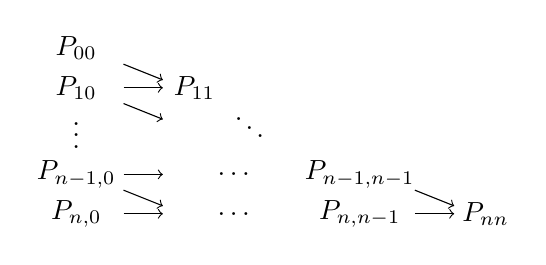
\begin{tikzpicture}[scale =1]
\node at (0,0) {$P_{00}$};
\node at (0,-0.5) {$P_{10}$};
\node at (1.5,-0.5) {$P_{11}$};
\node at (0,-1.6) {$P_{n-1,0}$};
\node at (0,-2.1) {$P_{n,0}$};
\node at (3.6,-1.6) {$P_{n-1,n-1}$};
\node at (3.6,-2.1) {$P_{n,n-1}$};
\node at (5.2,-2.1) {$P_{nn}$};
\node at (0,-1){$\vdots$};
\node at (2.2,-0.9){$\ddots$};
\node at (2,-1.6) {$\dots$};
\node at (2,-2.1) {$\dots$};
\draw[->] (0.6,-0.2) -- (1.1,-0.4);
\draw[->] (0.6,-0.5) -- (1.1,-0.5);
\draw[->] (0.6,-0.7) -- (1.1,-0.9);
\draw[->] (0.6,-1.6) -- (1.1,-1.6);
\draw[->] (0.6,-1.8) -- (1.1,-2);
\draw[->] (0.6,-2.1) -- (1.1,-2.1);
\draw[->] (4.3,-1.8) -- (4.8,-2);
\draw[->] (4.3,-2.1) -- (4.8,-2.1);
\end{tikzpicture}
\end{center}
\end{itemize}
